A robot has been developed to this end, however it still lacks the biological
component required for it to be a real cybernetic organism.
\subsubsection{Concept}
The concept of the cyborg is inspired by similar efforts such as
\cite{li_application_2015} and \cite{warwick paper}.
Fig \[?\] shows the basic premise: An in vitro neuron culture will be used to
control a robot in a closed loop system, making the robot an actual cyborg.
\subsubsection{Platform}
The cyborg 
\begin{figure}[h!]
    %\centering
    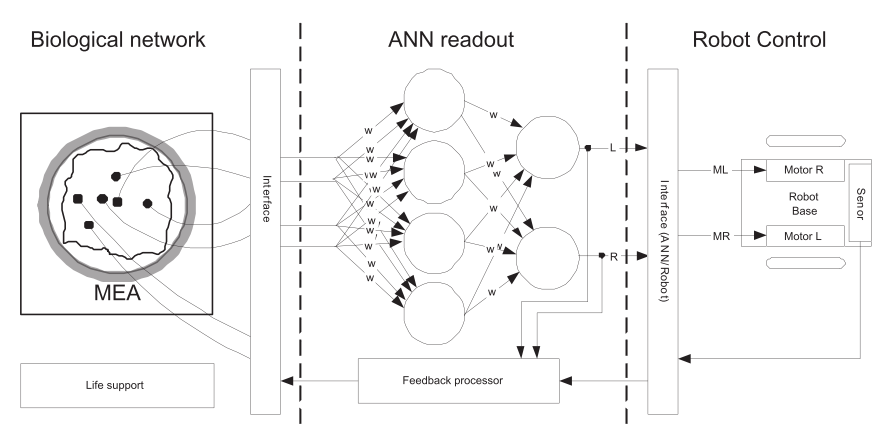
\includegraphics[width=\linewidth]{images/cyborg_overview.png}
    \caption{The gist of it..}
    \label{fig:cyborg_idea}
\end{figure}
\subsubsection{Growing NIV}
\subsubsection{A First Test}

%%% Local Variables:
%%% mode: latex
%%% TeX-master: "../main"
%%% End: